\chapter{Technical Solution}

In this section an overview of the design, architecture and distinctive features of the solution is given. Then, technical decisions are explained.



\section{Design \& Architecture}

The architecture of this project is designed to meet the requirements discussed in section \ref{problem}. First, a bird's eye view is given on where this recommender framework fits into existing systems. Then, the internal architecture of the framework is explained. Finally, distinctive features of this framework are introduced.

\subsection{Serviceoriented Architecture (SOA)}
\label{sol-design-soa}

\begin{figure}[ht]
    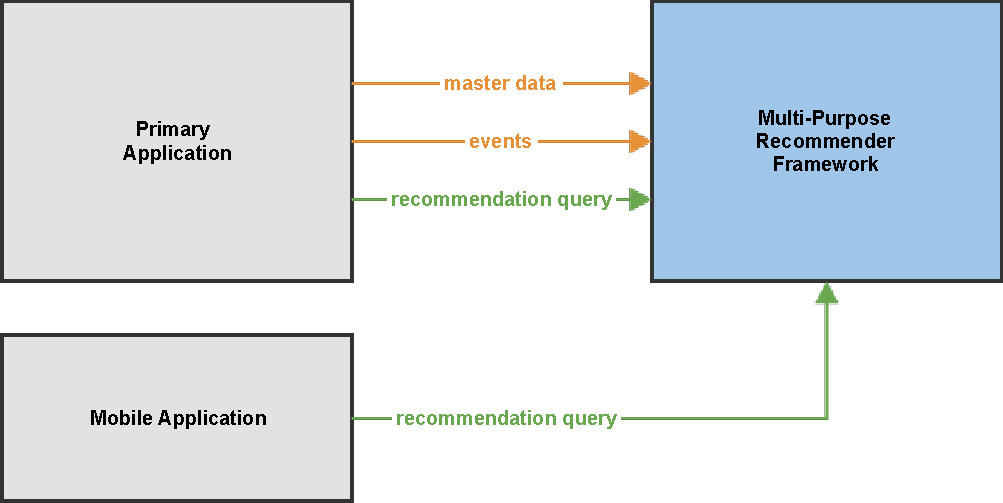
\includegraphics[width=0.7\textwidth,center]{solution/soa/soa.pdf}
    \caption[Service-Oriented Architecture (SOA)]{Service-Oriented Architecture (SOA). Orange arrows (\emph{master data} and \emph{event}) are \emph{notifications} whereas green arrows (\emph{recommendation query}) are \emph{queries} and expect a result.}
    \label{fig:soa}
\end{figure}

A \emph{service-oriented architecture (SOA)} is a software design pattern which is most suitable to meet the \emph{abstraction} requirement discussed in section \ref{problem-abstraction}. \emph{SOA} suggests to express features as services. This is true for features which are going to be available to other systems. Internal features are never to be exposed and allowed to be services. A \emph{service consumer} is a system using the service. \cite{erl08} identifies eight principles of \emph{SOA} of which I will elaborate:

\begin{description}
    \item[Standardised service contracts] is an expression of the service's purpose, capabilities and requirements -- such as mandatory parameters and data types. As long as the requirements are satisfied, the service agrees to fulfill its purpose.
    \item[Service loose coupling] makes sure that services have as few dependancies as possible.
    \item[Service abstraction] ensure that as much information as possible hidden and none except those described in the service contract are exposed.
    \item[Service reusability] assure that services are designed to be reused.
\end{description}

In figure \ref{fig:soa} a possible architecture of this project is shown. The framework is designed to serve more than one application or system component. The services accept requests from any source as long as they authorise with an access key. In the mentioned figure services are divided in two types -- \emph{notification} and \emph{query}. A \emph{notification} is a message relevant to the recommender framework and is simply acknowledged as received. A \emph{query} on the other hand expects a result. The framework will define three services:

\begin{description}
    \item[Master Data] enables service consumers to create, update or delete a data node in the framework. An identifier and type are mandatory fields. The service consumer is allowed to send any further features of the node which it thinks is relevant to the framework.
    \item[Event] accepts notifications about interactions or preferences between two or more nodes such as \emph{'X purchased Y and Z'}. The payload -- content of the message -- may contain a \emph{weight} which is a numeric value. It is useful for e.g. \emph{'X rated Y with 10'}.
    \item[Recommendation Query] requests recommendations for a specific \emph{recommendation model}. The recommendation model identifier is mandatory. A node identifier and type are only mandatory if the model excepts it. This is the only service which expects a result.
\end{description}

The recommendation framework only expects incoming requests (\emph{push strategy}) and has no outgoing communication at all.

\subsection{Multilayered Architecture}
\label{sol-design-layer}

\begin{figure}[ht]
    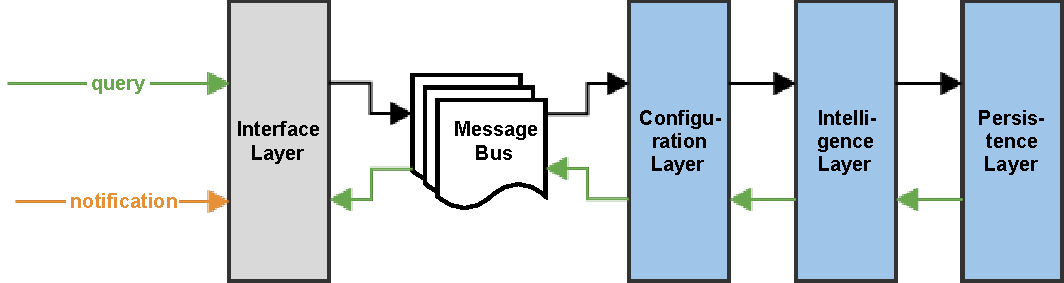
\includegraphics[width=\textwidth,center]{solution/layers/layers.pdf}
    \caption{Multilayered Architecture}
    \label{fig:layers}
\end{figure}

A multi-layered architecture is a software design pattern for software programs which suggests separating functionality in responsibility layers. This is popular way of abstracting functionality within a system.

Strictly speaking, the framework is divided into two subsystems: the \emph{application programming interface (API)} and \emph{recommender ecosystem}. These subsystems are connected with a message bus. The motivation of this differentiation is of a technical rather than logical manner. The subsystems have different kind of technical requirements and this division allows me to use the most appropriate technology for each. Another side effect are the advantages of a message bus which allows me to group and prioritise messages. \emph{Recommendation queries} may be processed by a dedicated resource whereas \emph{event} messages may have higher priority -- and should be processed sooner -- than \emph{master data} messages. However this makes no difference to the responsibilities, and is therefore not further considered in the specification of layers.

\subsubsection{Interface Layer}
\label{sol-design-layer-interface}

The interface layer is where services expose themselves to service consumers. Latter send requests to this layer. From a technical point of view this layer is implemented as an \emph{application programming interface (API)} via the \emph{hypertext transfer protocol (HTTP)} which is the foundation of data communication in the world wide web. The \emph{API} adopts the \emph{representational state transfer (REST)} style. An \emph{API} using \emph{REST} is called \emph{RESTful}. \citet{fielding00} -- who introduced \emph{REST} -- explains:

\begin{quotation}
    \small
    \emph{The name ``Representational State Transfer'' is intended to evoke an image of how a well-designed Web application behaves: a network of web pages (a virtual state-machine), where the user progresses through the application by selecting links (state transitions), resulting in the next page (representing the next state of the application) being transferred to the user and rendered for their use.}
\end{quotation}

Two concepts of \emph{REST} are important to understand: the use of \emph{uniform resource locator (URL)} and \emph{HTTP vocabulary}. The \emph{URL} provides a way to specify a resource -- in this case a service or node. The \emph{HTTP vocabulary} defines amongst others \emph{GET}, \emph{POST} and \emph{DELETE}. Combined a \emph{RESTful API} enables the access or modification of resources. E.g. to submit an event a \emph{POST} request to \emph{/events} is necessary. To delete a node with the identifier \emph{120} a \emph{DELETE} request to \emph{/nodes/120} is sufficient, whereas a \emph{GET} request to \emph{/recommendations/topseller} would return all recommendations for a recommendation model called \emph{topseller}. By using low-level \emph{HTTP} vocabulary the \emph{API} requires less documentation and explanation.

This layer acts as \emph{service broker} and \emph{security agent} at the same time. Latter is ensured by verifying the presence and correctness of an access key which is a random text. As a \emph{service broker} this layer validates the payload against mandatory fields and data types. Then, it offloads the message and submits it into the message bus for further processing. If the message is of the type \emph{notification} it acknowledges the request. If the message type is a \emph{query}, then it waits for a response from the message bus and returns that.

\subsubsection{Configuration Layer}
\label{sol-design-layer-config}

This layer is the heart of the multi-purpose recommender framework and targets to satisfy the multi-purpose and interoperability requirement (as defined in \ref{problem-multipurpose}). The motivation behind this layer is to empower operators -- who use this solution -- to set up a recommender system by configuration only. The configuration layer consists of two fundamental ideas: the \emph{recommendation model} and \emph{event} subsystems.

A \emph{recommendation model} is an instruction to the recommender to compute and how to compute recommendations. In the model configuration the recommender to be used is specified. An identifier allows service consumers to access recommendations for that particular model.

As mentioned in section \ref{sol-design-soa}, an event is an interaction or preference between two or more nodes such as \emph{'X purchased Y and Z'}. The event subsystem provides a mechanism to allow recommendation models to listen to events. When an event message is received, the subsystem will update listeners about it. This way recommendation models receive new data. One event can be interesting for more than one recommendation model. In a traditional architecture the primary application would need to update every single recommender system. However the event subsystem makes redundant API calls obsolete as only one message is sufficient, to update many recommendation models. Figure \ref{lst:recomodel-config} shows an example configuration.

\begin{listing}[ht]
    \xmlfile{listings/solution/recommendation.xml}
    \caption{Recommendation Model Configuration}
    \label{lst:recomodel-config}
\end{listing}

\subsubsection{Recommendation Layer}
\label{sol-design-layer-reco}

In the \emph{recommendation layer} the actual recommender algorithms will remain. These algorithms are called explicitly based on the recommender specified by the configuration layer. The recommender algorithms are going to be unaware of the nature of the data. In the contrary it will work based on the parameters fed by the configuration layer. Then, the algorithm will build its algorithm-specific query and use the persistance layer to fetch data and eventually return recommendations.

A distinctive feature of this framework will be the recommender plug-in subsystem. All recommenders will be designed as extensions. This subsystem will support extending the framework with new recommenders. This is actually a big potential to become a mechanism to define hybrid recommenders based on other recommenders in the framework and define a combination criterion (as discussed in section \ref{bg-tech-hybrid}). However most probably time would not permit to work on the latter.

\subsubsection{Persistance Layer}

This layer provides database abstraction components which will then allow any recommender system to access any of the supported storage systems.



\section{Technological Choices}

In this section I will discuss my choices in technology I want to use in this project.

\subsection{Application Programming Interface (API)}

The \emph{API} is the interface layer in this project and has almost none business logic. In that sense it is important to use a lightweight, thin solution. As discussed in \ref{sol-design-layer-config} I will use a \emph{RESTful} approach for the \emph{API}.

The \emph{API} will be built on the \emph{node.js} platform which makes use of \emph{Google Chrome}'s fast \emph{JavaScript} runtime and requires only a few lines of code to create a server. The \emph{API} will further use \emph{express} -- a web application framework for \emph{node.js}. \emph{express} is ideal for \emph{RESTful APIs} as it uses the \emph{HTTP} vocabulary as well. Figure \ref{lst:expressjs} illustrates a sample implementation of `\emph{GET} request to \emph{/recommendations/topseller}' mentioned in \ref{sol-design-layer-interface}. As visible in the figure the footprint of the implementation is very thin. As the \emph{API} has a specific format in \emph{express}, it is able to automatically generate \emph{API} documentation. Asynchronous processing capabilities will be accomplished with the \emph{node.js} module \emph{async.js}.

\begin{listing}[ht]
    \jsfile{listings/solution/express.js}
    \caption{Sample API for recommendations in \emph{express}}
    \label{lst:expressjs}
\end{listing}

The message format will be \emph{JavaScript Object Notation (JSON)} - a thinner alternative to \emph{extensible markup language (XML)} (listing \ref{lst:sample-json}).

\begin{listing}[ht]
    \jsonfile{listings/solution/example.json}
    \caption{Sample API message in \emph{JavaScript Object Notation (JSON)}}
    \label{lst:sample-json}
\end{listing}




\subsection{Message Bus}

The concept of the message bus was introduced in section \ref{sol-design-layer}. The main requirement for this message bus is that it implements the \emph{advanced message queuing protocol (AMQP)} -- an open standard which defines a minimum set of features in message buses. A popular, highly reliable message bus software which supports \emph{AMQP} is \emph{RabbitMQ}. It also provides a \emph{graphical user interface (GUI)} giving information about the current message flow. I have worked with \emph{RabbitMQ} in the past.

\subsection{Recommender Ecosystem}

This subsystem contains configuration, intelligence and persistence layers. It has the highest technical requirements amongst the solution as it needs to be performant and stable. Especially, the recommender algorithms will require a performant environment. In that sense dynamic scripting languages such as \emph{hypertext preprocessor (PHP)} or \emph{Python} are not my first choice. In fact a simple statically-typed, compiled language with concurrency capabilities is needed. 

My preferred candidate for this is \emph{Go} -- a language developed by \emph{Google} as an alternative to overcome limitations of the programming language \emph{C++}. The result is a language which is intendedly not adopting all patterns found in many programming languages such as overloading and pointers. The language aims to be simple, safe and free of misinterpretations by the compiler. It supports multithreading, CPU paralleling as well as asynchrony. Finally, it has a modern package management system which allows retrieving packages from the internet.

\subsubsection{Database Software}

The recommender ecosystem requires a powerful yet flexible database software. As pointed out in section \ref{sol-design-soa} a master data can have an arbitrary number of additional fields. To fulfill the \emph{ease of integration} requirement a schema management solution is not desired. Schema-less databases -- also known as \emph{NoSQL} -- might be of interest. \emph{NoSQL} databases are usually non-relational as well. However recommendations are very intensive in terms of relations (e.g. \emph{`X rated Y'}).

A potential solution are graph databases which understands \emph{nodes}, \emph{properties} and \emph{edges}. A \emph{node} is a reference with an identifier. An \emph{edge} is a path -- thus relation -- from one \emph{node} to another. A \emph{property} can be attached to \emph{nodes} as well as \emph{edges}. Latter is useful for weighted relations such as \emph{`X rated Y with 10'}. Figure \ref{fig:graph} shows a sample graph. Graph databases have further advantages especially in querying distant \emph{nodes} via other \emph{nodes}. With regard to figure \ref{fig:graph}, an example query could be to fetch all groups people, who Alice knows, are members of.

\begin{figure}[ht]
    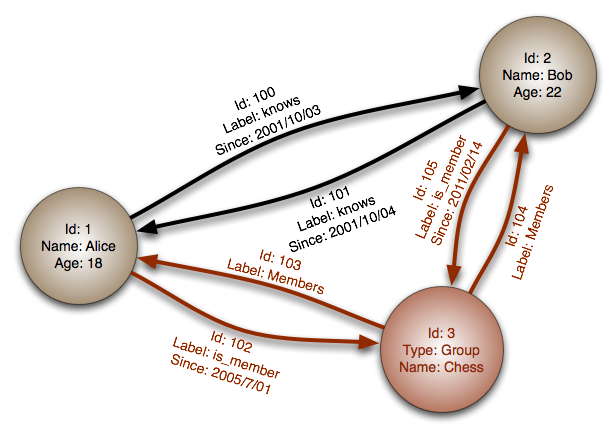
\includegraphics[width=0.7\textwidth,center]{solution/tech/graph.png}
    \caption[Simple Graph in a Graph Database]{Simple Graph in a Graph Database. Source: Creative Commons.}
    \label{fig:graph}
\end{figure}

\subsection{Others}

A \emph{version control management (VCS)} namely \emph{git} will be used throughout the project. \emph{Git} is a distributed \emph{VCS} which is amongst others faster and more flexible than other \emph{VCS} such as \emph{Subversion}. The \emph{git} repository -- and therefore the source code -- will be hosted on \emph{BitBucket} to have a backup of the project anytime.

For server health and performance monitoring I will use the \emph{software as a service (SAAS)} solution \emph{NewRelic}. It also allows to analyse specific low performing or faulty requests. This will be very useful during testing and evaluation of the solution.

\begin{figure}[ht]
    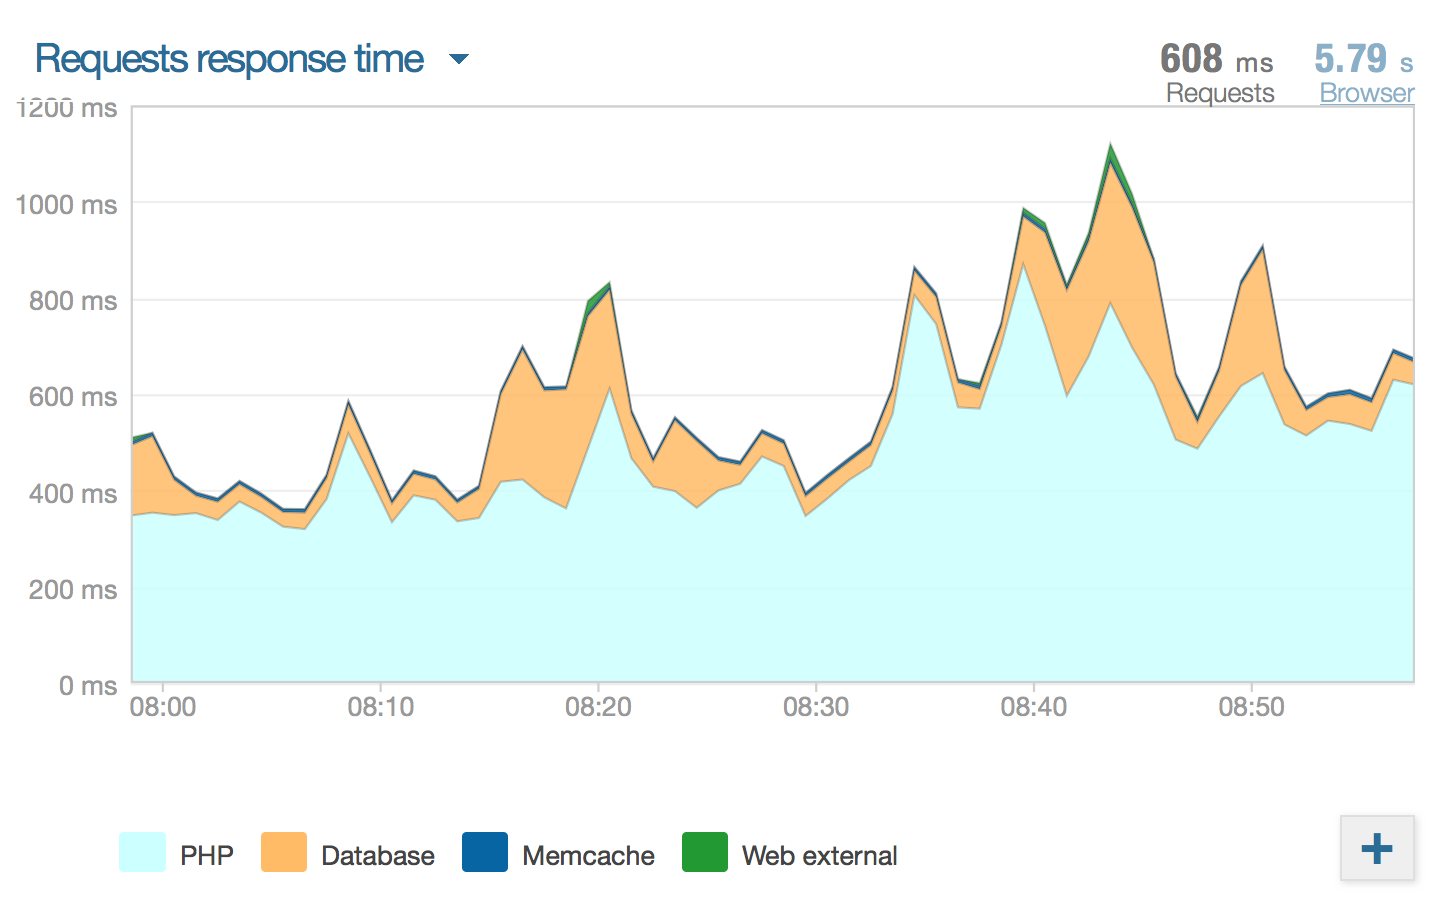
\includegraphics[width=0.7\textwidth,center]{solution/tech/newrelic.png}
    \caption{Monitoring with NewRelic}
    \label{fig:newrelic}
\end{figure}

Finally, a virtualisation solution called \emph{VirtualBox} will be used to set up all technical and vendor requirements within a virtual machine. This prevents conflicts with dependencies on the workstation especially if versions differ. When submitting the project the virtual machine will be packaged to provide a seamless demo setup for examination.